\documentclass[11pt]{article}

\usepackage[margin=1in]{geometry}
\usepackage{graphicx}
\usepackage{booktabs}
\usepackage{array}
\usepackage{tabularx}
\usepackage{hyperref}
\usepackage{xcolor}
\usepackage{enumitem}
\usepackage{caption}
\usepackage{amsmath}
\usepackage{float}
\usepackage{listings}

\hypersetup{colorlinks=true,linkcolor=blue,urlcolor=blue,citecolor=blue}
\lstset{basicstyle=\ttfamily\small,breaklines=true,frame=single,columns=fullflexible}
\setlength{\tabcolsep}{4pt}
\renewcommand{\arraystretch}{1.12}
\newcolumntype{Y}{>{\raggedright\arraybackslash}X}
\newcolumntype{Z}[1]{>{\raggedright\arraybackslash}p{#1}}

\title{Scene Understanding Model Optimization via DL Compiler}
\author{RepNeXt-M5 ADE20K Optimization Project}
\date{June 2026}

\begin{document}
\maketitle

\begin{abstract}
This project optimizes a scene-understanding model for edge inference using DL compiler techniques. The workload is RepNeXt-M5 semantic segmentation on ADE20K. It is intentionally non-trivial: native Raspberry Pi 5 inference takes 4222.626 ms/frame, so optimization has visible user value. We built three tracks: Intel CPU, Raspberry Pi 5 ARM CPU without Coral, and Raspberry Pi 5 ARM CPU with two Google Coral USB Edge TPUs. TVM was central for graph analysis, Relay-level partition/fusion experiments, operator inspection, and understanding which computation could become compiler-friendly. The final deployable paths also required ONNX, TensorFlow Lite/LiteRT, and the Edge TPU compiler because TVM does not provide a direct export route from an optimized Relay graph to an Edge-TPU-compilable \texttt{.tflite}. The best accuracy-valid edge result is the Raspberry Pi 5 ARM CPU LiteRT 256 model: 351.377 ms/frame and 0.2135 ADE20K mIoU, a 12.0x speedup over native RPi5 PyTorch. The best TPU compiler result is a w48 RepNeXt-style full graph at 192 input resolution: 84.130 ms/frame, 960/960 operations mapped to one Coral TPU subgraph, and only 57.75 KiB off-chip streaming. This TPU artifact proves the full pipeline can be made accelerator-computable, but it still needs distillation and quantization-aware training to recover accuracy.
\end{abstract}

\section{Introduction}

Scene understanding is useful in robotics, surveillance, assistive devices, and industrial monitoring because decisions must often be made near the camera. Edge inference reduces network latency, keeps video local for privacy, and allows operation when connectivity is unreliable. The difficulty is that semantic segmentation is expensive: a naive RepNeXt-M5 run on Raspberry Pi 5 is several seconds per frame.

The goal was not just to run a tiny model. The goal was to show that DL compiler optimization can turn a meaningful model into a practical edge demo. Therefore we focused on compiler-visible improvements: graph partitioning, operator fusion opportunities, quantization, layout rewriting, accelerator mapping, and runtime scheduling.

\section{Terms Used in This Report}

\begin{itemize}[leftmargin=*]
  \item \textbf{mIoU:} mean Intersection over Union. For each semantic class, IoU is the overlap between predicted pixels and ground-truth pixels divided by their union. mIoU averages this over ADE20K classes. Higher is better.
  \item \textbf{Pixel accuracy:} fraction of valid pixels whose class is predicted correctly. It is easier to score high than mIoU because large classes dominate.
  \item \textbf{Logits:} raw per-class scores before choosing the final class. For ADE20K segmentation, a tensor such as $64\times64\times150$ means 150 class scores at each low-resolution pixel.
  \item \textbf{Dynamic-range quantization:} TFLite method that quantizes weights but keeps most activations in floating point. It is not valid for Coral TPU, but it preserved accuracy well on RPi5 ARM CPU.
  \item \textbf{Full INT8 quantization:} weights and activations are both INT8. This is required by Coral TPU, but post-training INT8 caused a large accuracy drop in RepNeXt.
  \item \textbf{CPU prefix/suffix:} parts of the model that remain on the Raspberry Pi ARM CPU before or after a TPU subgraph. They are a problem when they dominate end-to-end latency.
\end{itemize}

\section{Hardware and Software}

\begin{table}[H]
\centering
\caption{Evaluation targets and comparison rule.}
\small
\begin{tabularx}{\textwidth}{Z{0.22\textwidth}Y Y}
\toprule
Track & Hardware & Comparison in this report \\
\midrule
Intel CPU & 11th Gen Intel Core i5-1135G7 @ 2.40 GHz & Intel native vs Intel compiled CPU pipeline \\
RPi5 ARM CPU w/o Google Coral TPU x2 & Raspberry Pi 5 BCM2712 ARM CPU & RPi5 native PyTorch vs RPi5 LiteRT/TFLite \\
RPi5 ARM CPU w/ Google Coral TPU x2 & Raspberry Pi 5 plus two Coral USB Edge TPUs & RPi5 hybrid TPU vs improved TPU-compiled artifacts \\
\bottomrule
\end{tabularx}
\end{table}

All conversion and compilation were done on the local Intel computer. The Raspberry Pi 5 was used as the runtime target only; compiled binaries were copied to it.

\begin{table}[H]
\centering
\caption{Compiler and runtime stack.}
\small
\begin{tabularx}{\textwidth}{Z{0.22\textwidth}Y}
\toprule
Component & Role \\
\midrule
TVM & Relay import, graph inspection, partition/fusion experiments, CPU compiler experiments, and guidance for graph rewrites \\
ONNX & Portable graph exchange from PyTorch \\
OpenVINO & Intel CPU compiled execution for graph partitions \\
TensorFlow Lite / LiteRT & Deployable RPi5 CPU runtime and required input format for Coral compilation \\
onnx2tf & Practical ONNX-to-SavedModel/TFLite conversion route \\
Edge TPU compiler & Final Coral USB TPU binary compiler for fully quantized INT8 \texttt{.tflite} files \\
\bottomrule
\end{tabularx}
\end{table}

\section{Why TVM Was Important}

TVM was not only a failed export attempt; it shaped the optimization. We used TVM/Relay to reason about the graph at compiler level: what could be fused, which partitions were expensive, which operators blocked export, and where CPU prefix/suffix execution remained. This analysis led to the main design decisions:

\begin{itemize}[leftmargin=*]
  \item replace partial offload with full-graph compilation where possible;
  \item avoid unsupported operators and rewrite depthwise-shaped convolutions;
  \item reduce activation and parameter footprint so the Edge TPU compiler can map the graph;
  \item benchmark partitions separately before building end-to-end demos.
\end{itemize}

However, TVM could not be the whole production pipeline for Coral. The Edge TPU compiler accepts only fully quantized INT8 TensorFlow Lite files. TVM can optimize Relay and generate CPU/GPU code, but this project needed an Edge-TPU-compilable \texttt{.tflite}. There was no reliable route from a TVM-optimized Relay graph back to a Coral-valid \texttt{.tflite}. Therefore the final deployable chain became:

\begin{lstlisting}
PyTorch RepNeXt
 -> ONNX
 -> onnx2tf / TensorFlow SavedModel
 -> TensorFlow Lite INT8 or dynamic-range model
 -> Edge TPU compiler when targeting Coral
\end{lstlisting}

TVM still contributed at the DL-compiler level by informing graph partitioning, fusion feasibility, operator compatibility, and the decision to move from partial acceleration to full-graph compiler-clean artifacts.

\section{Implementation}

\subsection{Track 1: Intel CPU}

The Intel CPU track tested native PyTorch against compiled CPU execution on the same i5-1135G7 machine. We split RepNeXt into stage01, middle, and suffix partitions. ONNX partitions were compiled with OpenVINO, and the middle partition was also tested through LiteRT/TFLite. TVM LLVM experiments with the Tiger Lake target were used to evaluate compiler-lowered partition execution and to inspect graph-level optimization opportunities.

The best Intel path used persistent compiled objects:

\begin{lstlisting}
input -> OpenVINO stage01 -> quantize
      -> LiteRT INT8 middle -> dequantize
      -> OpenVINO suffix -> logits
\end{lstlisting}

\begin{table}[H]
\centering
\caption{Intel CPU result.}
\small
\begin{tabularx}{\textwidth}{Y Z{0.18\textwidth} Z{0.18\textwidth}}
\toprule
Intel CPU variant & Mean latency & Speedup \\
\midrule
PyTorch baseline & 3972.223 ms & 1.00x \\
\texttt{torch.compile} full model & 2608.011 ms & 1.52x \\
OpenVINO + LiteRT persistent pipeline & 2210.749 ms & 1.80x \\
\bottomrule
\end{tabularx}
\end{table}

\subsection{Track 2: Raspberry Pi 5 ARM CPU w/o Google Coral TPU x2}

The RPi5 CPU-only track produced the best accuracy-valid demo. The first attempt accelerated only a middle partition, but this left expensive prefix/suffix computation. The better solution was to compile the whole graph at a lower input resolution and keep the output as logits:

\begin{lstlisting}
RGB 256
 -> full RepNeXt graph, dynamic-range LiteRT/XNNPACK
 -> 64x64x150 logits
 -> upsample and overlay
\end{lstlisting}

Accuracy was recovered by keeping tanh-GELU instead of replacing it with ReLU, choosing 256 input resolution instead of 96, and using dynamic-range quantization instead of full INT8 activation quantization.

\begin{table}[H]
\centering
\caption{Raspberry Pi 5 ARM CPU result.}
\small
\begin{tabularx}{\textwidth}{Y Z{0.18\textwidth} Z{0.18\textwidth}Y}
\toprule
RPi5 ARM CPU variant & Latency & Accuracy & Note \\
\midrule
Native PyTorch 512 & 4222.626 ms & reference & full model baseline \\
Middle TFLite hybrid 512 & 3652.424 ms & visual pipeline & only 1.10x faster \\
Dynamic-range LiteRT 256 & 351.377 ms & 0.2135 mIoU & 12.0x faster; best accuracy-valid demo \\
Float16 LiteRT 256 & 422.435 ms & 0.2155 mIoU & accurate but slower \\
\bottomrule
\end{tabularx}
\end{table}

\subsection{Track 3: Raspberry Pi 5 ARM CPU w/ Google Coral TPU x2}

The Coral track required every accelerated operation to be in a fully quantized INT8 \texttt{.tflite}. The early hybrid model compiled only the middle segment:

\begin{lstlisting}
RGB 512 -> RPi5 ARM CPU prefix -> Coral TPU middle
        -> RPi5 ARM CPU suffix -> logits
\end{lstlisting}

This was not enough because the TPU middle took only 29 ms while the RPi5 ARM CPU prefix and suffix took several seconds. We then tried tiling at 256, 128, and 64, full low-resolution graph compilation, depthwise TFLite patching, transpose/concat folding, tanh-GELU preservation, and structural shrinking.

The strongest TPU compiler artifact was a smaller RepNeXt-style student:

\begin{lstlisting}
embed_dim = [48, 96, 192, 384]
depth     = [4, 4, 8, 2]
fpn_out   = 96
head_ch   = 64
input     = 192
\end{lstlisting}

This graph maps completely to the Coral TPU and removes CPU prefix/suffix fallback.

\begin{table}[H]
\centering
\caption{Raspberry Pi 5 ARM CPU w/ Google Coral TPU x2 result.}
\small
\begin{tabularx}{\textwidth}{Y Z{0.16\textwidth} Z{0.2\textwidth}Y}
\toprule
TPU variant & Latency & TPU mapping & Status \\
\midrule
Middle-only TPU hybrid 512 & 4064.330 ms & middle only & CPU prefix/suffix dominate \\
Full RepNeXt 96 Edge TPU & 184.880 ms & all ops mapped & fast but inaccurate; high streaming \\
w48 192 Edge TPU & 84.130 ms & 960/960 ops, 1 subgraph & best compiler-clean TPU artifact; needs QAT/distillation \\
w48 256 Edge TPU & 246.770 ms & 985/1001 ops & 16 CPU transpose fallbacks \\
\bottomrule
\end{tabularx}
\end{table}

\begin{figure}[H]
\centering
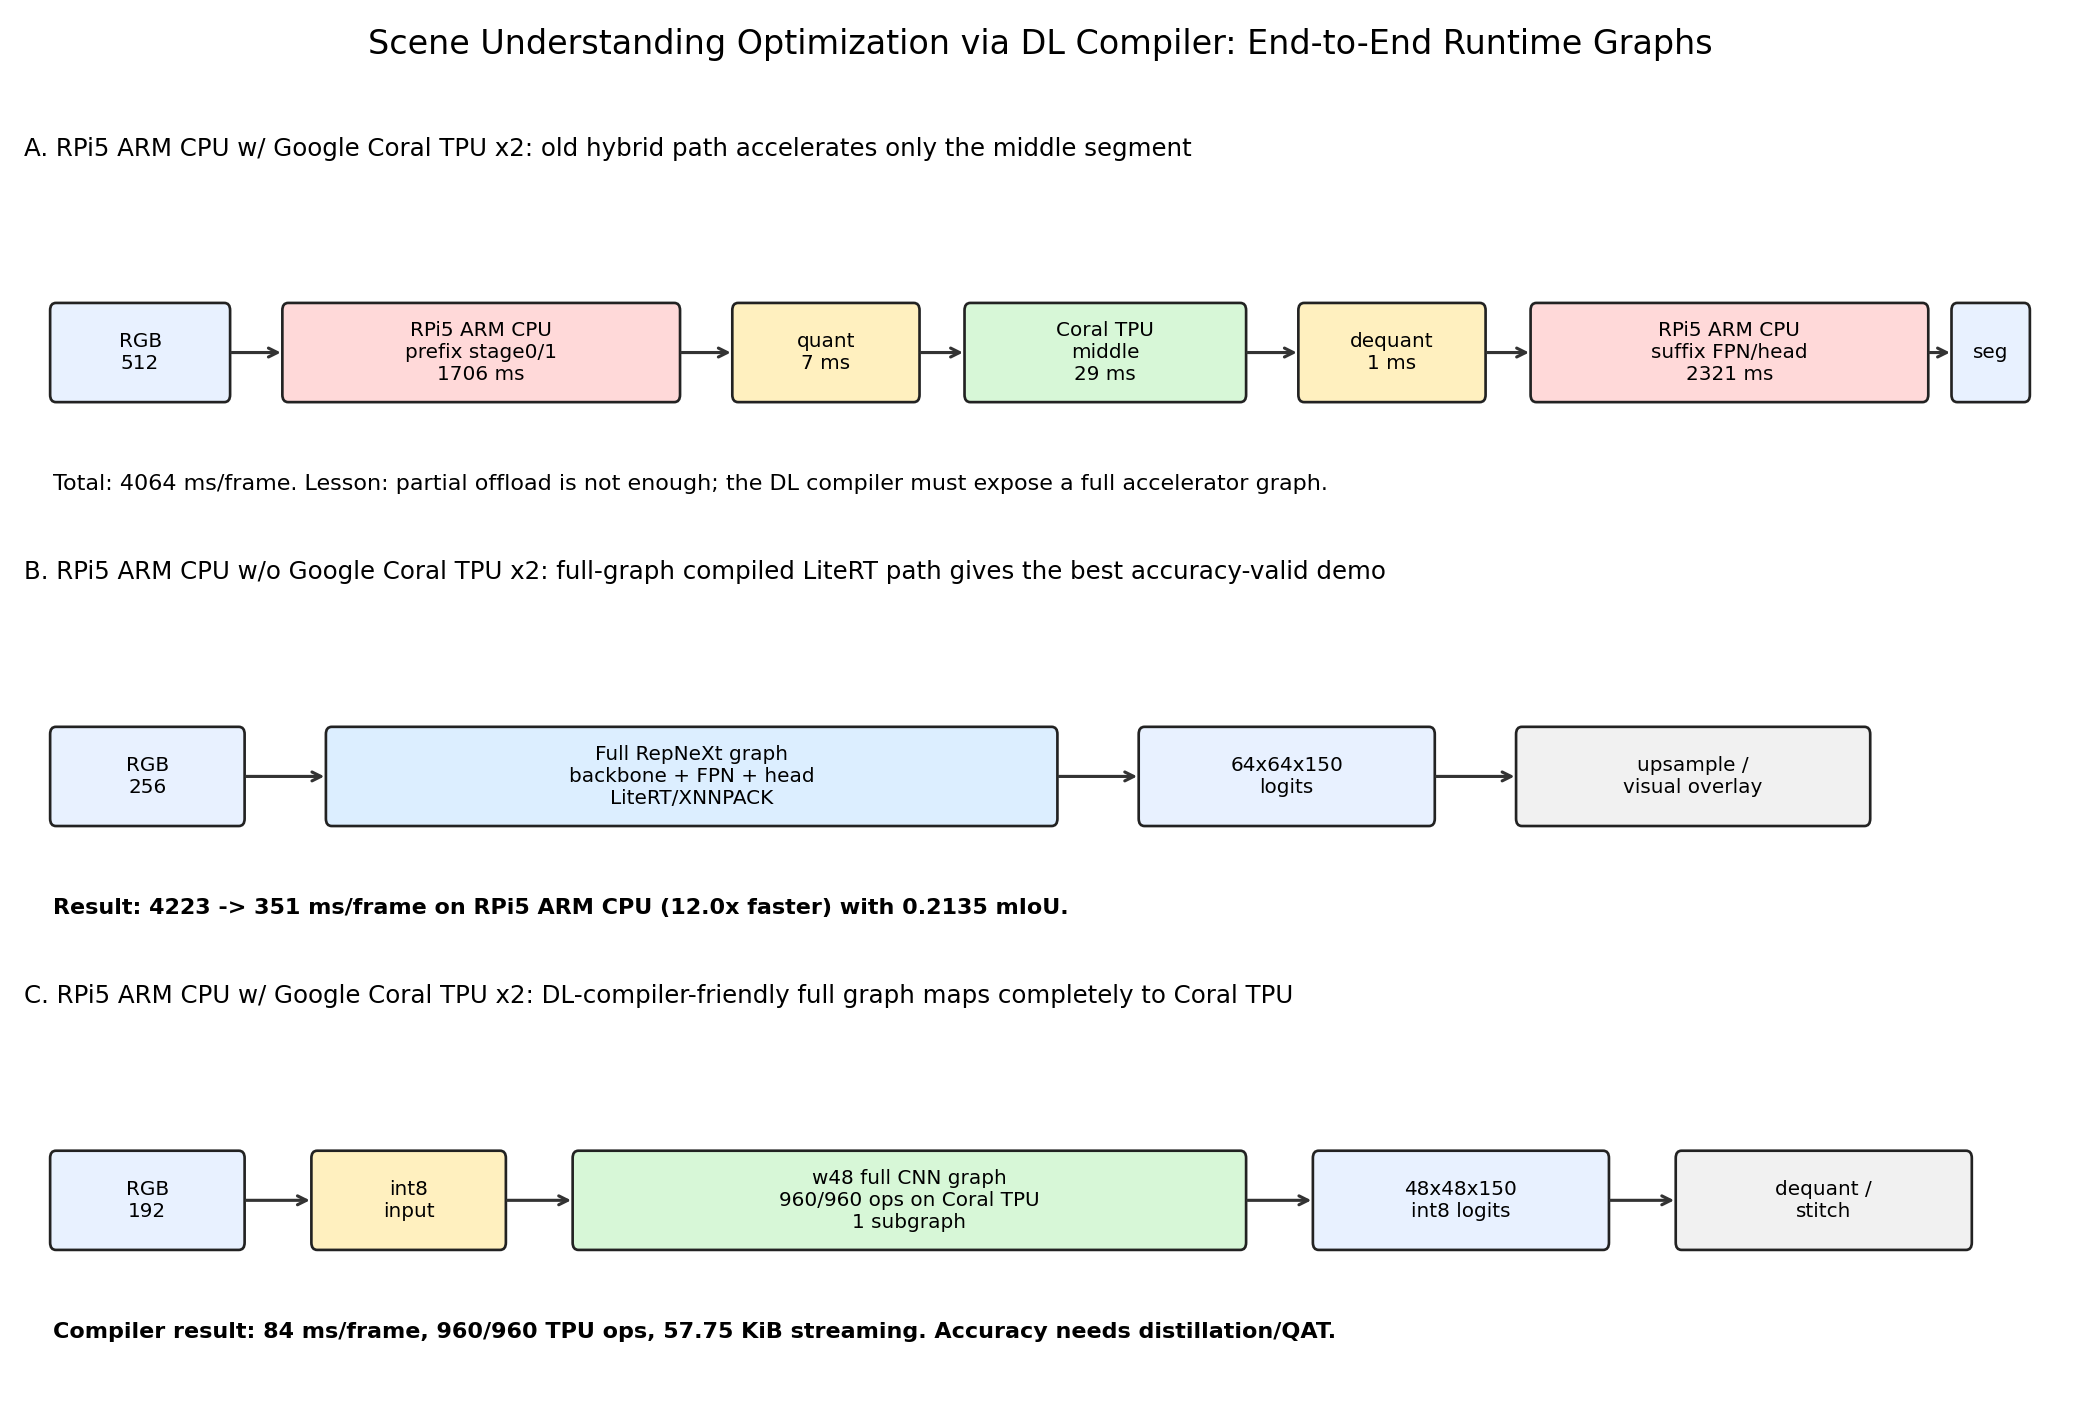
\includegraphics[width=\textwidth]{demo/runtime_graphs/end_to_end_runtime_graphs.png}
\caption{Implementation-level runtime graphs. The old Coral path still has RPi5 ARM CPU prefix/suffix work. The CPU-only LiteRT path compiles the whole graph for RPi5 ARM CPU. The w48 Coral path is the compiler-clean target where the full CNN graph maps to Coral TPU.}
\end{figure}

\section{Evaluation}

\subsection{Track-Level Latency and Accuracy Evaluation}

Each graph below compares latency and accuracy side by side within one hardware track. The same color always refers to the same model inside a graph. Accuracy is ADE20K val40 mIoU. For partitioned compiler pipelines, the plotted accuracy is the measured val40 accuracy of the same model family used by that pipeline.

\begin{figure}[H]
\centering
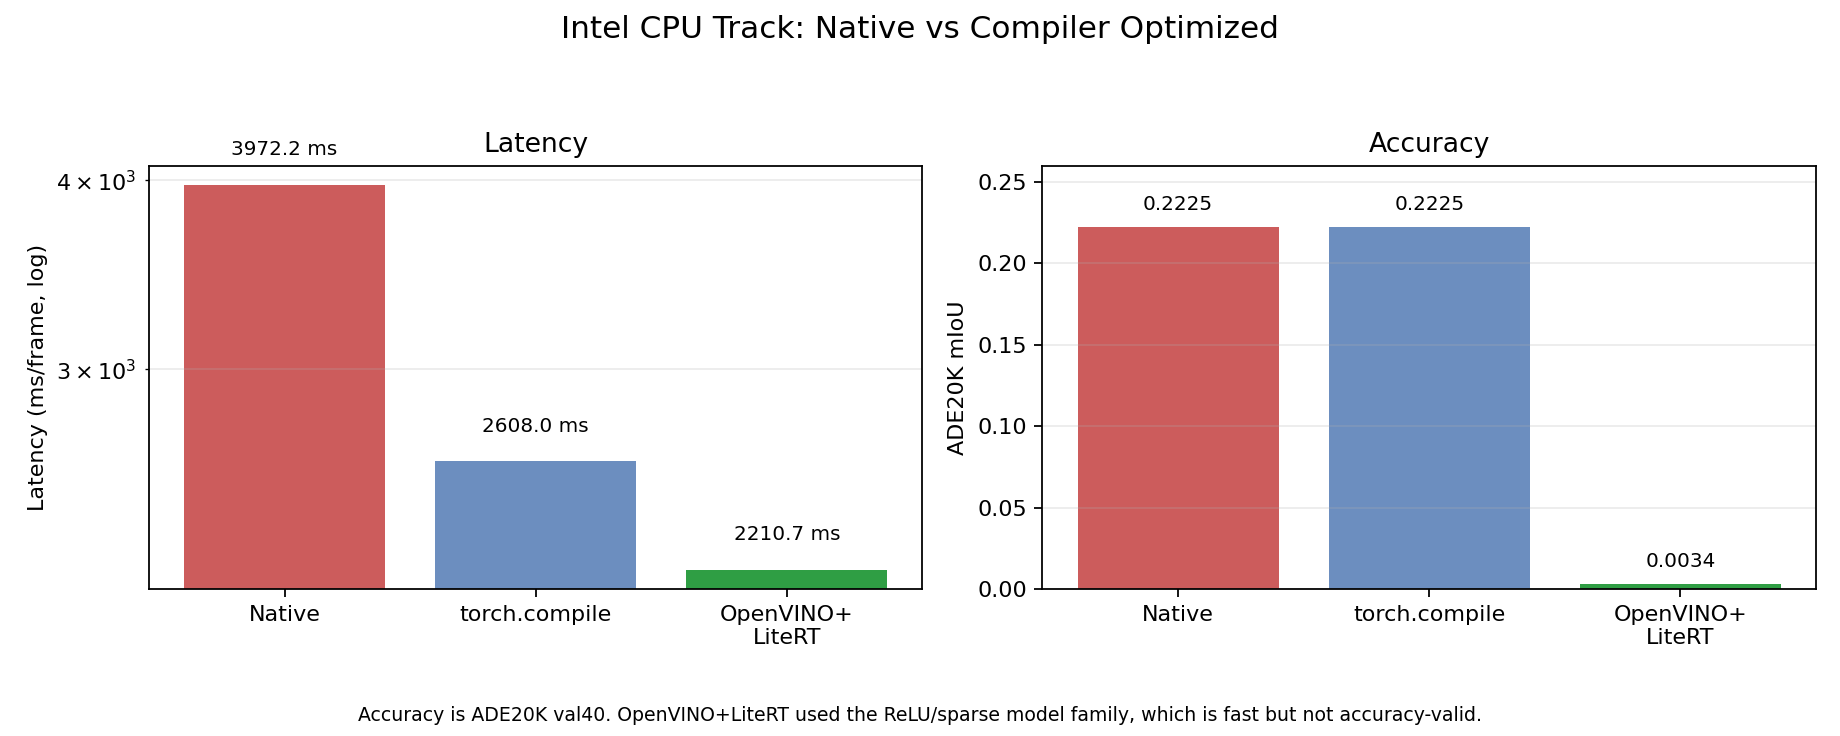
\includegraphics[width=\textwidth]{demo/runtime_graphs/intel_cpu_latency_accuracy.png}
\caption{Intel CPU track. \textbf{Native} is full PyTorch on Intel CPU. \textbf{torch.compile} is the full model compiled by PyTorch's compiler stack and preserves model semantics. \textbf{OpenVINO+LiteRT} is the fastest partitioned DL-compiler pipeline, but it used the ReLU/sparse model family; the measured val40 accuracy for that model family is only 0.0034 mIoU.}
\end{figure}

\begin{figure}[H]
\centering
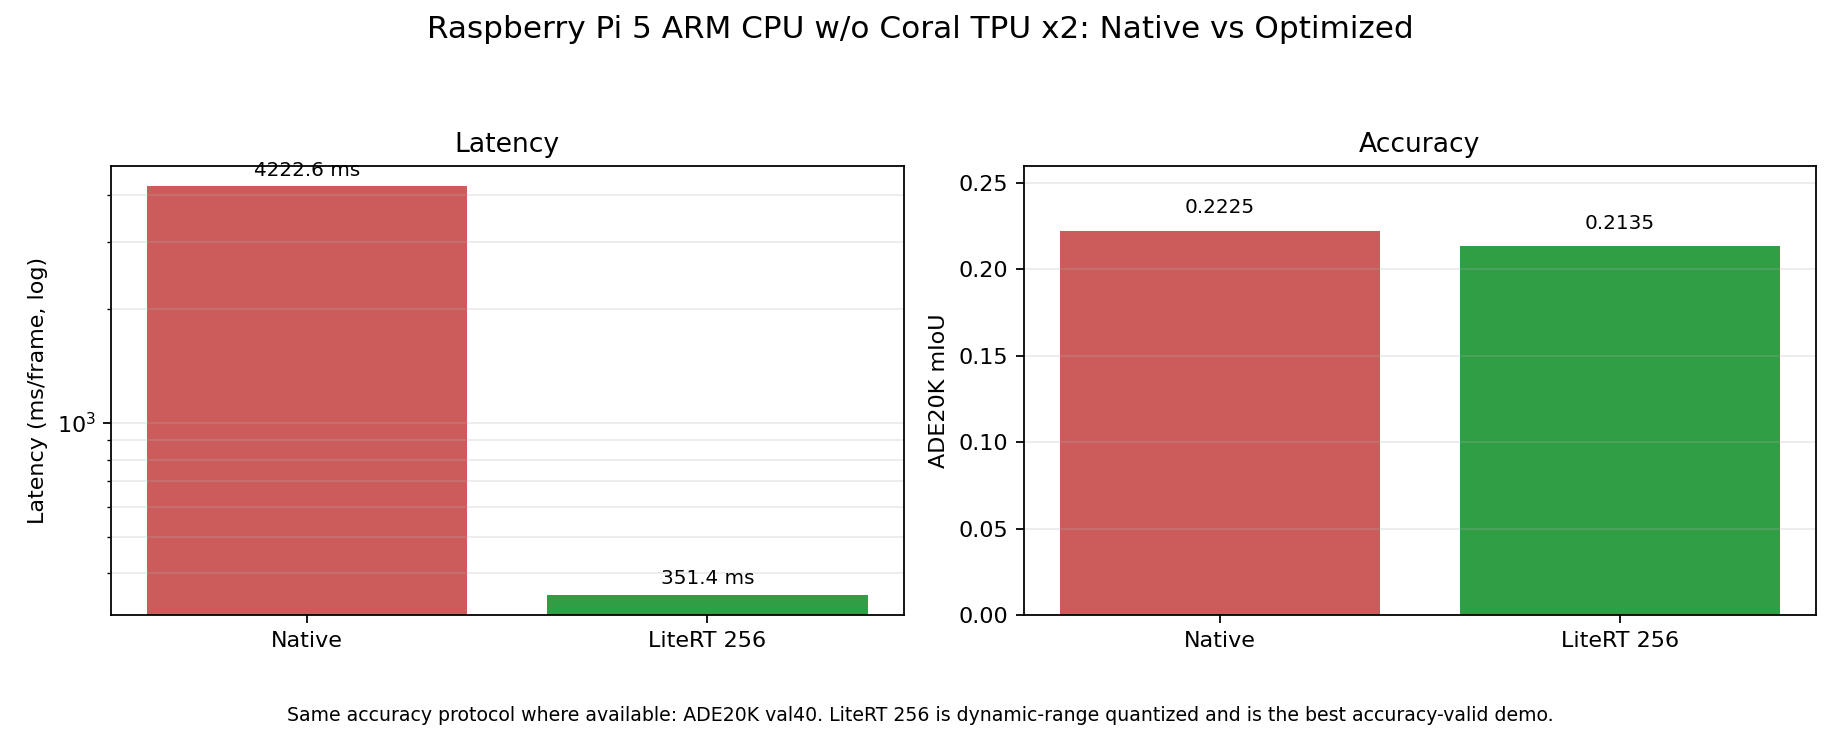
\includegraphics[width=\textwidth]{demo/runtime_graphs/rpi5_cpu_latency_accuracy.png}
\caption{Raspberry Pi 5 ARM CPU track without Coral TPU. \textbf{Native} is full PyTorch 512. \textbf{LiteRT 256} is the dynamic-range full-graph TFLite/LiteRT model at 256 input resolution. It is the strongest accuracy-valid demo: 12.0x faster with only a small mIoU drop from 0.2225 to 0.2135 under the same val40 protocol.}
\end{figure}

\begin{figure}[H]
\centering
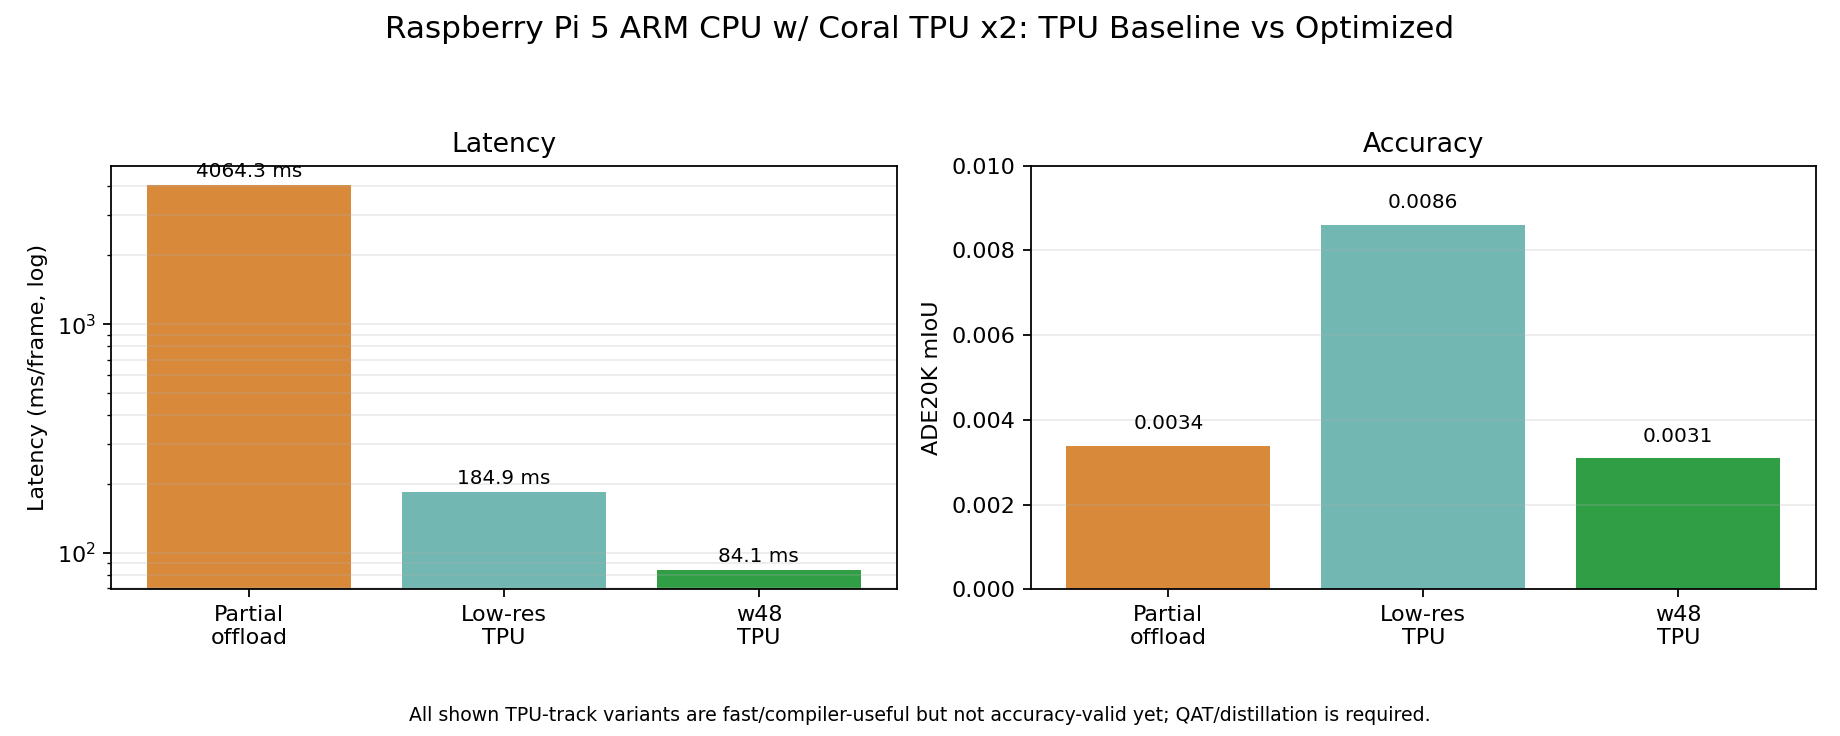
\includegraphics[width=\textwidth]{demo/runtime_graphs/coral_tpu_latency_accuracy.png}
\caption{Raspberry Pi 5 ARM CPU with Coral TPU x2 track. \textbf{Partial offload} is the old hybrid path where only the middle segment ran on Coral and the rest used the ReLU/sparse model family. \textbf{Low-res TPU} is the full RepNeXt low-resolution INT8 TPU path. \textbf{w48 TPU} is the compiler-clean shrunk model with 960/960 ops mapped to Coral. The TPU latency result is strong, but all current TPU-track accuracies are too low without QAT/distillation.}
\end{figure}

\subsection{Accuracy Evaluation}

Accuracy is evaluated as model-output quality, not as a hardware speed measurement. To avoid wrong comparisons, the main table below uses one protocol: ADE20K validation subset of 40 images, the same label mapping, and the same mIoU/pixel-accuracy computation. The names are intentionally simple: \textbf{Native} means the original full PyTorch model, \textbf{LiteRT 256} means the optimized RPi5 CPU deployable, \textbf{Low-res TPU} means the older low-resolution full INT8 TPU-compatible model, and \textbf{w48 TPU} means the shrunk compiler-clean TPU model.

\paragraph{How mIoU is calculated.}
For each ADE20K class, we count true-positive pixels, predicted pixels, and ground-truth pixels. The class IoU is:

\[
\mathrm{IoU}_c = \frac{\mathrm{TP}_c}{\mathrm{GT}_c + \mathrm{Pred}_c - \mathrm{TP}_c}.
\]

mIoU is the mean of this value over classes that appear in the validation subset. This is stricter than pixel accuracy. A model can produce visually plausible large regions such as sky, wall, floor, or road, but still get low mIoU if it misses small objects, predicts the wrong ADE20K fine-grained class, or shifts boundaries. ADE20K has 150 classes, so confusing similar categories is heavily penalized.

\begin{table}[H]
\centering
\caption{Accuracy comparison using the same ADE20K val40 protocol where the model can be evaluated end-to-end.}
\small
\begin{tabularx}{\textwidth}{Y Y Z{0.12\textwidth} Z{0.12\textwidth} Y}
\toprule
Easy name & Method used & mIoU & Pixel acc. & Meaning \\
\midrule
Native & PyTorch GELU, 512 input & 0.2225 & 0.7894 & reference model under val40 \\
LiteRT 256 & Tanh-GELU, dynamic-range quantization, 256 input & 0.2135 & 0.7874 & best no-training deployable \\
LiteRT 256 float16 & Tanh-GELU, float16 compression, 256 input & 0.2155 & 0.7895 & slightly more accurate, slower than dynamic-range \\
LiteRT 256 full INT8 & Tanh-GELU, full post-training INT8, 256 input & 0.0027 & 0.0427 & activation quantization collapses logits \\
Low-res TPU & Tanh-GELU, full INT8, 96 input & 0.0086 & 0.2521 & fast but not accuracy-valid \\
w48 TPU & shrunk w48 full INT8 model, 192 input & 0.0031 & 0.2007 & compiler-clean but not trained enough \\
ReLU/sparse compiler family & ReLU replacement and sparse-equivalent downsample & 0.0034 & 0.1142 & explains low accuracy for OpenVINO+LiteRT and partial-offload paths \\
\bottomrule
\end{tabularx}
\end{table}

\begin{figure}[H]
\centering
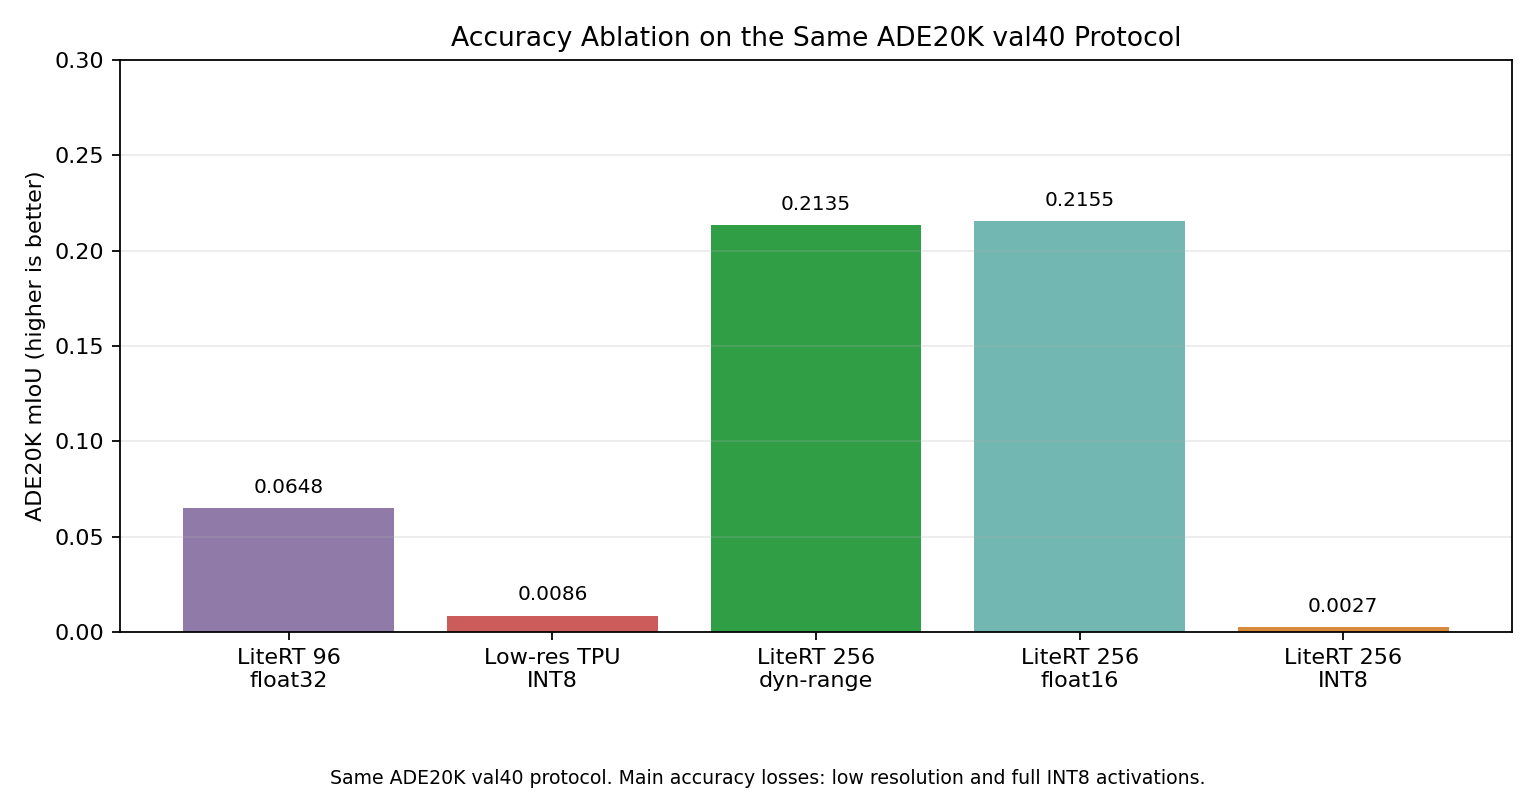
\includegraphics[width=0.92\textwidth]{demo/runtime_graphs/accuracy_ablation_miou.png}
\caption{Accuracy ablation using the same ADE20K val40 protocol. The accuracy drop is mainly caused by too-low input resolution and full INT8 activation quantization. Dynamic-range and float16 at 256 resolution preserve much more accuracy.}
\end{figure}

\paragraph{Why the TPU mIoU is poor.}
The current TPU artifacts are constrained by Coral hardware. Coral requires fully quantized INT8 execution, and the compiler rejects many larger full-resolution graphs because of large activation tensors and memory limits. Therefore the TPU track had to use low-resolution inputs, full INT8 activations, or a structurally shrunk w48 model. These choices make the graph computable on the Edge TPU, but they remove information that segmentation accuracy needs. In particular, full post-training INT8 activation quantization collapses RepNeXt logits, and low resolution removes small objects and boundaries. The result is that the TPU track is a strong \emph{compiler feasibility and latency} result, but not yet an accuracy-valid segmentation model.

\paragraph{Complementary evidence.}
mIoU remains the main quantitative metric, but it is not the only useful evidence for a demo. Pixel accuracy and qualitative overlays show whether the model preserves coarse scene layout. This is why the 256 dynamic-range LiteRT model is a good advisor demo: it keeps pixel accuracy near the native model (0.7874 vs 0.7894), keeps mIoU close to native (0.2135 vs 0.2225), and the overlay in Fig.~\ref{fig:demo-256} shows visually coherent segmentation. For the TPU track, the correct claim is narrower: the graph runs fast and maps to Coral, while QAT/distillation is required before its qualitative output can be treated as reliable.

The model names mean the following. \textbf{Tanh-GELU} is the activation approximation kept to match the original GELU-trained RepNeXt behavior. \textbf{LiteRT 96} and \textbf{LiteRT 256} are full-graph TFLite/LiteRT logits models at 96 or 256 input resolution. \textbf{Dynamic-range} means only weights are quantized, so it runs on RPi5 ARM CPU but cannot run on Coral TPU. \textbf{Full INT8} means weights and activations are INT8, which is required by Coral TPU but caused severe post-training accuracy loss.

We separately ran a small 5-image PyTorch diagnostic to isolate activation replacement. It should not be mixed with the val40 table above. In that diagnostic, original GELU PyTorch 512 gave 0.2582 mIoU, tanh-GELU PyTorch 512 gave 0.2585 mIoU, and ReLU PyTorch 512 gave 0.0027 mIoU. This shows that ReLU substitution was invalid for this pretrained model, while tanh-GELU preserved the original behavior.

\begin{figure}[H]
\centering
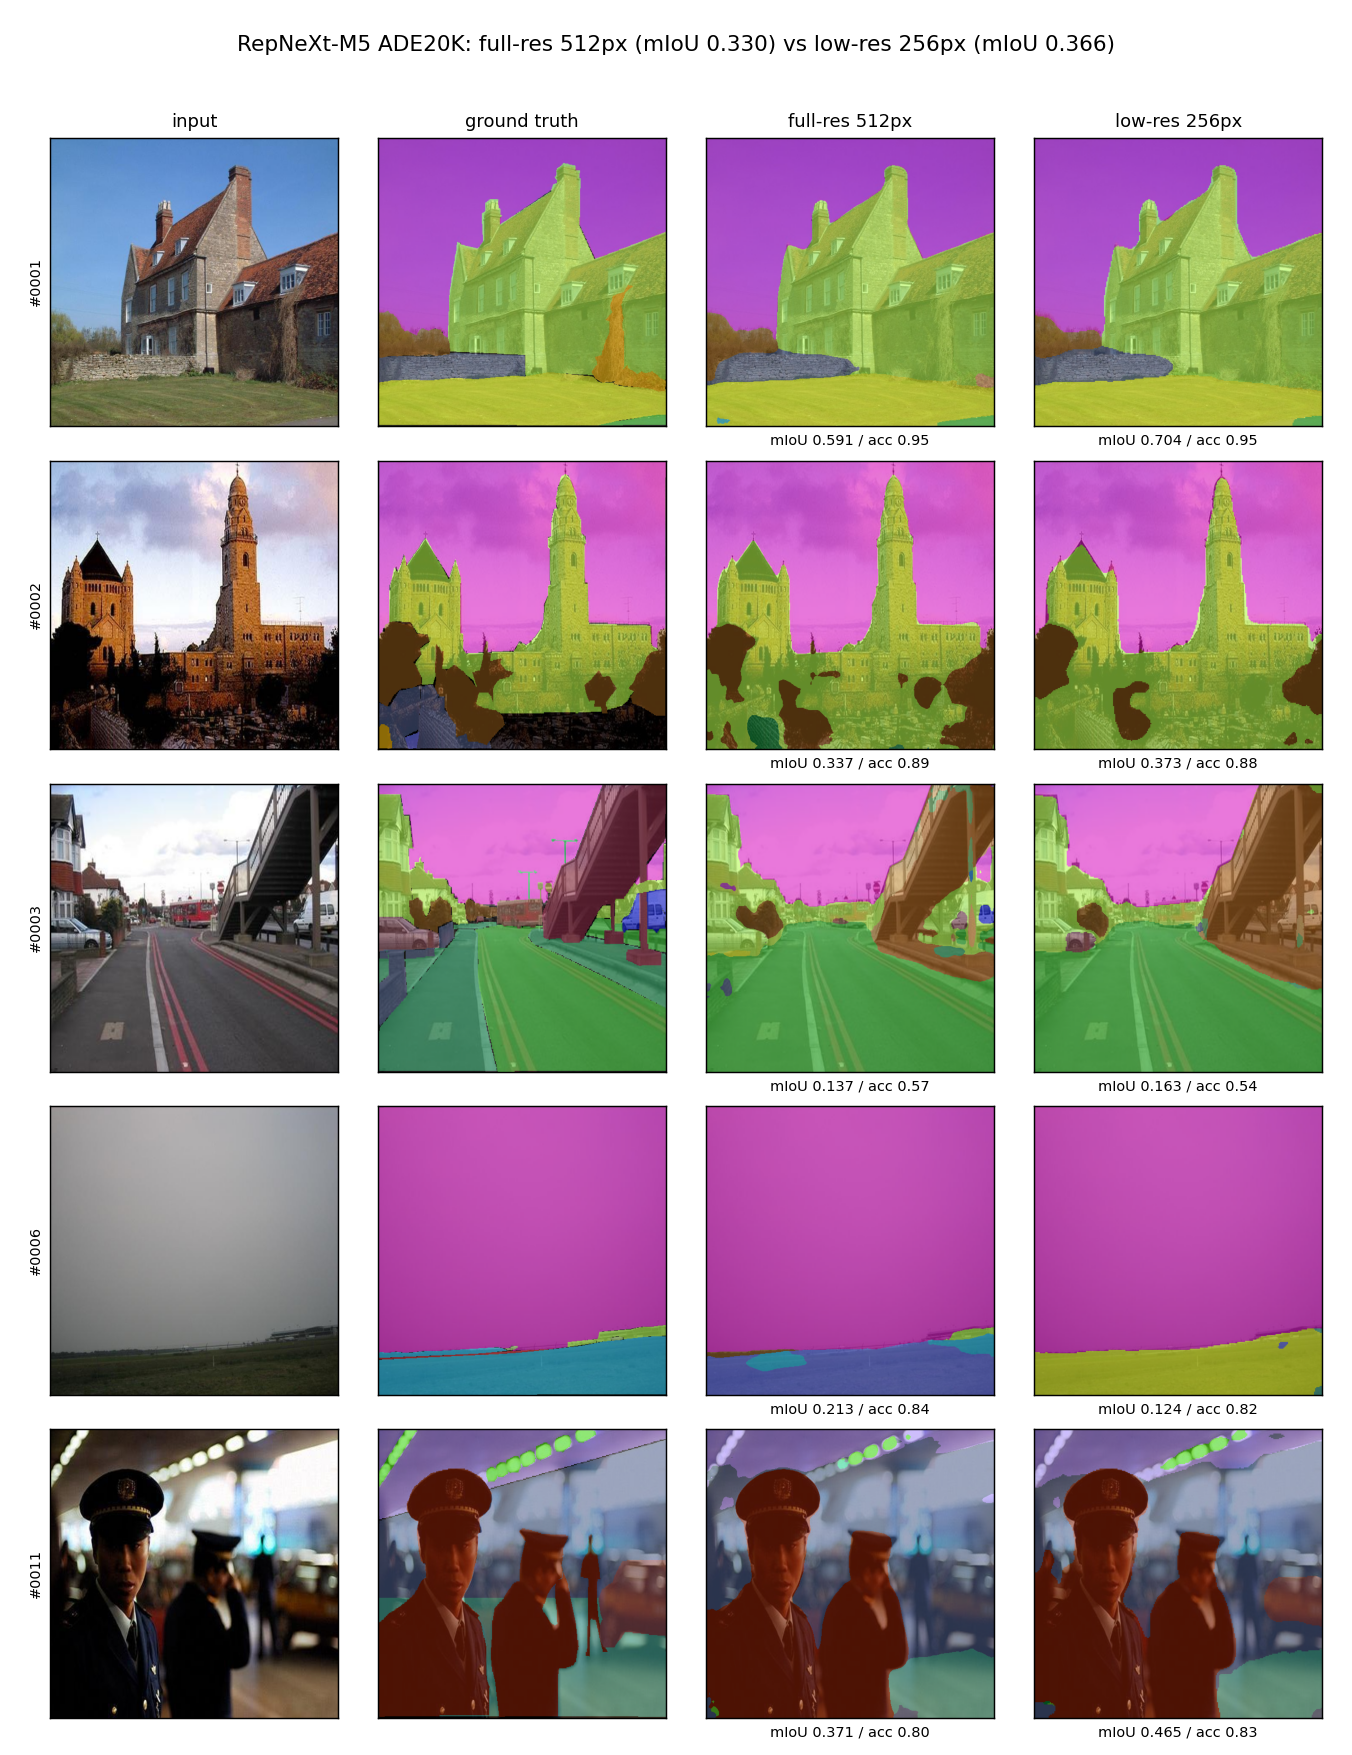
\includegraphics[width=\textwidth]{demo/seg_compare/fullres512_vs_fixed256.png}
\caption{Demo output comparison. The 256 dynamic-range model preserves the main scene layout while reducing RPi5 latency from 4222.626 ms to 351.377 ms.}
\label{fig:demo-256}
\end{figure}

\begin{figure}[H]
\centering
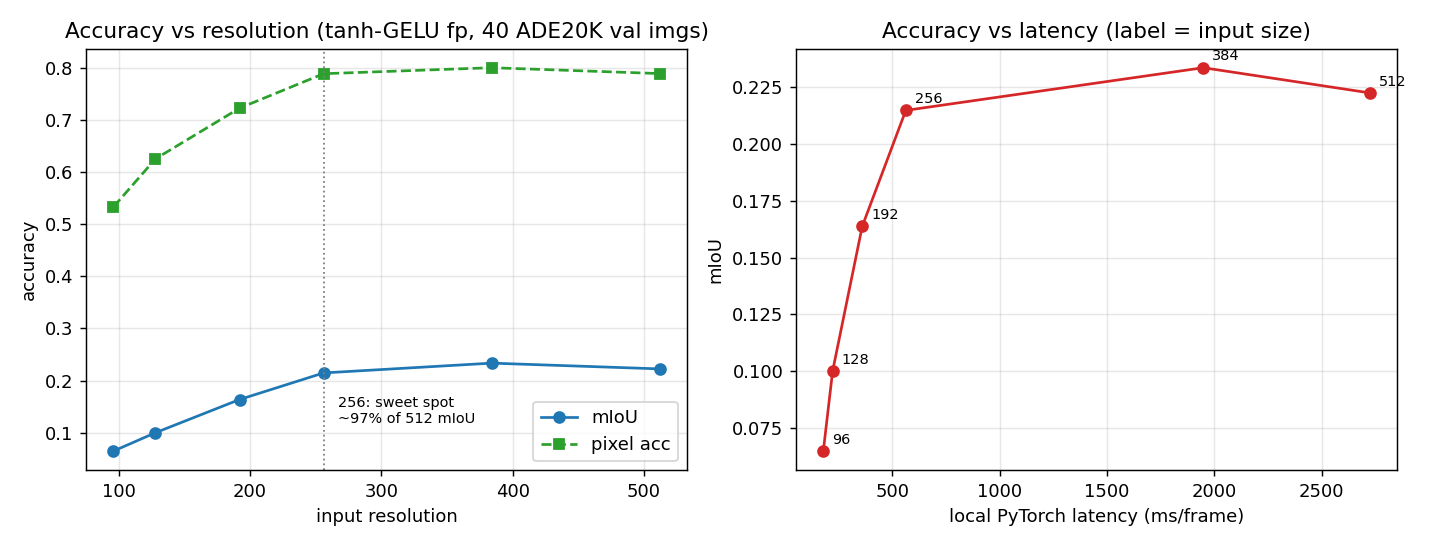
\includegraphics[width=0.85\textwidth]{demo/seg_compare/resolution_curve.png}
\caption{Resolution sweep. The 256 input is the practical accuracy/latency knee for the no-training CPU demo.}
\end{figure}

\section{Difficulties}

The main difficulties were practical compiler and hardware constraints:

\begin{itemize}[leftmargin=*]
  \item \textbf{TVM export gap:} TVM could optimize/analyze Relay graphs, but could not export an optimized graph as Coral-valid INT8 \texttt{.tflite}. This forced the ONNX/onnx2tf/TFLite/Edge-TPU-compiler route.
  \item \textbf{Edge TPU activation limits:} many full-size RepNeXt variants failed due to large activation tensors.
  \item \textbf{Strict INT8 requirement:} Coral does not run dynamic-range or float16 TFLite. It needs fully quantized INT8 models.
  \item \textbf{Tensor layout limits:} transpose-heavy and large 3D/4D tensor patterns caused CPU fallback or compiler failure.
  \item \textbf{Memory bandwidth and parameter cache:} full RepNeXt 96 mapped to TPU but streamed roughly 21--22 MiB per inference; the w48 model reduced this to 57.75 KiB.
  \item \textbf{USB and concurrency:} two Coral USB TPUs help throughput only when independent work exists. One frame mapped to one graph invocation does not automatically become twice as fast.
  \item \textbf{Runtime configuration:} old \texttt{tflite\_runtime} could not load newer op versions; newer LiteRT initially conflicted with PyCoral through NumPy version changes.
\end{itemize}

\section{Limitations and Further Study}

The best accuracy-valid result currently runs on RPi5 ARM CPU, not Coral. This is not just an implementation accident: it follows from the Coral constraints. The Edge TPU cannot accept the larger float/dynamic-range graphs that preserve accuracy, and it cannot execute the large-activation full-resolution RepNeXt graph directly. The best Coral graph is compiler-clean but needs training to regain accuracy. Full post-training INT8 quantization collapses the RepNeXt activations, so the next step is quantization-aware training plus distillation from the full RepNeXt teacher.

Methods considered but not finished include:

\begin{itemize}[leftmargin=*]
  \item \textbf{Quantization-aware training:} needed for INT8 Coral accuracy.
  \item \textbf{Knowledge distillation:} needed to make the w48 student accurate.
  \item \textbf{Structured pruning:} useful because Coral executes dense INT8 and benefits from fewer channels.
  \item \textbf{Zero skipping:} less useful on Coral because unstructured sparsity is not directly exposed.
  \item \textbf{Redundant computation skipping for video:} reuse static regions or run segmentation at lower temporal frequency.
  \item \textbf{Cache-conscious scheduling and memory mapping:} promising for CPU targets through TVM scheduling and for Coral through smaller parameter working sets.
  \item \textbf{Layout-aware transpose folding:} likely to remove the remaining 16 CPU transpose fallbacks in the w48 256 artifact.
\end{itemize}

\section{Conclusion}

The project achieved a clear optimization result. The best deployable accuracy-valid model reduces Raspberry Pi 5 ARM CPU latency from 4222.626 ms/frame to 351.377 ms/frame, a 12.0x speedup, while keeping 0.2135 ADE20K mIoU. The TPU track also achieved the key compiler objective: a full RepNeXt-style CNN graph that maps completely to Coral TPU with no CPU prefix/suffix fallback, running at 84.130 ms/frame.

The main lesson is that DL compiler optimization is necessary but not sufficient by itself. TVM and compiler analysis identified the right graph transformations and exposed why partial offload failed. The final Coral deployment still required the TensorFlow Lite and Edge TPU compiler toolchain because Coral accepts only INT8 \texttt{.tflite}. To make the 84 ms TPU path production-quality, the remaining work is training: distillation and quantization-aware training for the compiler-clean w48 model.

\end{document}
